% Copyright 2026 Sreeram Anil
% SPDX-License-Identifier: CC-BY-4.0
% =============================================================================
%  Joint state / parameter adaptive observer
% =============================================================================
\chapter{Adaptive Observer for Joint State and Parameter Estimation (AdaptiveObserver)}
\label{ch:adaptiveobserver}

\section*{At a glance}
\begin{tabular}{@{}l>{\raggedright\arraybackslash}p{0.76\textwidth}@{}}
Family & Deterministic observers \\
Header & \texttt{include/estkit/observers/adaptive\_observer.hpp} \\
Registered name & \texttt{AdaptiveObserver} \\
State dimension & $n_x = 4$ states $+$ $n_\theta = 2$ parameters $+$ an $n_x\times n_\theta$ sensitivity \\
Cost per step & $\mathcal{O}(n_x n_\theta)$ plus $2n_\theta$ model evaluations; $\approx 0.9\,\mu$s/step measured \\
Primary references & \cite{kreisselmeier1977,zhang2002adaptiveobserver,zhang2001forgetting,ioannou1996robust} \\
SOH capability & yes --- reports $\hat{Q}_{Ah}$ through \texttt{with\_capacity} \\
\end{tabular}

\section{Motivation and aerospace/BMS relevance}
Every observer in this family so far has assumed the model is right and the disturbances are what
is wrong.  For a battery that is backwards.  The dominant error source over the life of a pack is
that the model parameters drift: the capacity fades, the series resistance grows, and both do so
by tens of percent over a few hundred cycles \cite{wang2011cyclelife,schmalstieg2014aging}.  No
amount of disturbance estimation recovers from a $15\,\%$ capacity error, because that error is
proportional to the instantaneous current and therefore not a disturbance in any useful sense.

An adaptive observer estimates the state and the parameters together.  Kreisselmeier
\cite{kreisselmeier1977} gave the first exponentially convergent construction; Zhang
\cite{zhang2002adaptiveobserver} generalised it to MIMO linear time-varying systems in the form
used here, with a filtered sensitivity (``regressor'') matrix propagated through the observer
dynamics.  For a BMS the payoff is twofold: the SOC estimate stops being biased by the parameter
error, and the parameter estimate itself is the state of health.  An eVTOL operator who can read
$\hat{Q}_{Ah}$ after every flight has a maintenance signal that no amount of SOC filtering
provides.

\section{Problem statement and assumptions}
Plant \eqref{eq:lue-plant-f}--\eqref{eq:lue-plant-h} where $f$ and $h$ depend on an unknown
constant parameter vector $\vtheta\in\real^{n_\theta}$ (the model's \texttt{params()}; for the
cell, $\vtheta = [Q_{Ah},\ R_0]^\T$).
\begin{assumption}[Persistency of excitation]\label{as:ad-pe}
The output sensitivity $\bm{\Omega}_k$ defined in \eqref{eq:ad-omega} satisfies
$\sum_{k=m}^{m+N}\bm{\Omega}_k^\T\bm{\Omega}_k \succeq \alpha\mI$ for some $\alpha>0$, $N$ and
all $m$.
\end{assumption}
\begin{assumption}[Parameter range]\label{as:ad-range}
$\vtheta$ lies in a known box around the nominal $\vtheta_0$ supplied at reset.
\end{assumption}

\section{Derivation}

\subsection{Relative parameterisation}
The cell's parameters differ by three orders of magnitude ($Q_{Ah}\approx5$\,Ah,
$R_0\approx12$\,m$\Omega$).  A single adaptation gain cannot serve both, and per-parameter gains
would have physical units.  The implementation therefore adapts the \emph{relative deviation}
$\bm{\phi}$ defined by
\begin{equation}
\vtheta = \vtheta_0\odot(\bm{1}+\bm{\phi}) , \qquad
\bm{\phi}\in[\phi_{\min},\phi_{\max}]^{n_\theta} ,
\label{eq:ad-rel}
\end{equation}
so every sensitivity, gain and bound in the algorithm is dimensionless.  The projection interval
is the numerical form of \Cref{as:ad-range}; $[-0.45,0.45]$ is used here, i.e. $\pm45\,\%$ of
nominal.

\subsection{Sensitivities}
With $\vtheta_0$ fixed, define
\begin{equation}
\bm{\Psi}_k = \frac{\partial f}{\partial\bm{\phi}}\Big|_{\xhat_k,\vu_k}\in\real^{n_x\times n_\theta} ,
\qquad
\bm{\Phi}_k = \frac{\partial h}{\partial\bm{\phi}}\Big|_{\xhat_k,\vu_k}\in\real^{n_y\times n_\theta} .
\label{eq:ad-sens}
\end{equation}
These are obtained by central differences through \texttt{Model::set\_params}, using the chain
rule $\partial/\partial\phi_i = \theta_{0i}\,\partial/\partial\theta_i$.  No analytic derivative
is required of the model, which is what keeps the observer generic.

\subsection{Zhang's filtered regressor}
The key object is the \emph{filtered sensitivity} $\bm{\Upsilon}\in\real^{n_x\times n_\theta}$,
which propagates the accumulated effect of a parameter error on the state estimate.  Zhang
\cite{zhang2002adaptiveobserver} defines it by
$\bm{\Upsilon}_{k+1} = (\mA-\mL\mC)\bm{\Upsilon}_k + \bm{\Psi}_k - \mL\bm{\Phi}_k$; split across
the predictor--corrector cycle this becomes
\begin{align}
\bm{\Upsilon}^-_k &= \mA\,\bm{\Upsilon}^+_{k-1} + \bm{\Psi}_{k-1} , \label{eq:ad-ups-pred}\\
\bm{\Omega}_k     &= \mC\,\bm{\Upsilon}^-_k + \bm{\Phi}_k , \label{eq:ad-omega}\\
\bm{\Upsilon}^+_k &= \bm{\Upsilon}^-_k - \mL\,\bm{\Omega}_k . \label{eq:ad-ups-upd}
\end{align}
$\bm{\Omega}_k\in\real^{n_y\times n_\theta}$ is the sensitivity of the \emph{output residual} to
the parameter error, and it is the correct regressor: to first order,
\begin{equation}
r_k = y_k - h(\xminus_k,\vu_k) \simeq -\mC\veps^-_k - \bm{\Omega}_k\,\big(\hat{\bm{\phi}}-\bm{\phi}\big) .
\label{eq:ad-regress}
\end{equation}

\subsection{Update law and the state/parameter coupling}
A normalised gradient step on \eqref{eq:ad-regress},
\begin{equation}
\bm{\Delta}_k = \frac{\bm{\Gamma}\,\bm{\Omega}_k^\T\, \bm{r}_k}{1 + \norm{\bm{\Omega}_k}_F^2/\nu}
 - \lambda_\sigma\,\hat{\bm{\phi}}_{k-1} ,
\qquad
\hat{\bm{\phi}}_k = \Pi\big[\hat{\bm{\phi}}_{k-1} + \bm{\Delta}_k\big] ,
\label{eq:ad-update}
\end{equation}
with $\bm{\Gamma} = \diag(\gamma_i)$, normalisation constant $\nu$, optional
$\sigma$-modification $\lambda_\sigma$ \cite{ioannou1996robust} and projection $\Pi$ onto the box.
The state update carries an extra term:
\begin{equation}
\xplus_k = \xminus_k + \mL\,\bm{r}_k + \bm{\Upsilon}^-_k\,\bm{\Delta}_k .
\label{eq:ad-state}
\end{equation}
The last term is Zhang's state/parameter coupling.  Its role is to correct the state estimate for
the instantaneous change of the parameter estimate: without it the two error dynamics are coupled
in both directions and stability requires a small-gain argument; with it the joint error system
becomes block-triangular,
\begin{equation}
\begin{bmatrix}\veps_k\\ \tilde{\bm{\phi}}_k\end{bmatrix}
=\begin{bmatrix}(\mI-\mL\mC)\mA & \bm{0}\\ \ast & \mI - \bm{\Gamma}\bm{\Omega}^\T\bm{\Omega}/(1+\cdot)\end{bmatrix}
\begin{bmatrix}\veps_{k-1}\\ \tilde{\bm{\phi}}_{k-1}\end{bmatrix} + \text{noise} ,
\label{eq:ad-triangular}
\end{equation}
so the state error converges at the observer's own rate and the parameter error converges
exponentially whenever $\bm{\Omega}$ is persistently exciting (\Cref{as:ad-pe})
\cite[Thm.~1]{zhang2002adaptiveobserver}.  The implementation applies the \emph{projected}
increment in \eqref{eq:ad-state}, so the coupling stays consistent with the parameter actually
used.

\subsection{Excitation and identifiability for the cell}
\label{sec:ad-pe}
It is worth checking \Cref{as:ad-pe} concretely, because it determines what can and cannot be
identified.
\begin{itemize}[nosep]
\item $R_0$: $\partial h/\partial R_0 = -i$, so $\Omega_{R_0} = -\theta_{0,R_0}\,i$.  This is
directly excited by every current change and is large ($-66$\,mV per unit relative deviation at
$i = 5.5$\,A).  $R_0$ is strongly identifiable.
\item $Q_{Ah}$: $h$ does not depend on $Q_{Ah}$ at all, so $\Phi_{Q}=0$ and the whole regressor
comes through $\bm{\Upsilon}$: $\partial f_{\soc}/\partial\phi_Q = +\eta\dt\,i/(3600Q) =
3\times10^{-5}$ per step at $5.5$\,A, accumulated and damped by \eqref{eq:ad-ups-upd}.  The
resulting $\Omega_Q$ is of order $10^{-2}$, three orders of magnitude below $\Omega_{R_0}$.
\end{itemize}
This is why a single adaptation gain does not work and why the registered configuration uses
$\gamma_{Q} = 0.1$ and $\gamma_{R_0} = 0.5$: the weakly excited parameter must be adapted
\emph{more slowly}, not faster, so that the gradient step is not dominated by the strongly excited
one during the transient.  Both regressors share a DC component (the current is always positive
during a discharge), so $Q_{Ah}$ and $R_0$ are partially confounded; the measured result
(\Cref{sec:ad-results}) is that they separate correctly when only one of them is wrong and drift
together when the scenario is ambiguous.

\section{Algorithm}
\begin{algorithm}[H]
\caption{AdaptiveObserver --- one sampling period}
\begin{algorithmic}[1]
\Require $\xplus_{k-1}$, $\hat{\bm{\phi}}_{k-1}$, $\bm{\Upsilon}^+_{k-1}$, $\vu_{k-1}$, $y_k$, $\vu_k$
\State $\bm{\Psi}_{k-1}\gets \partial f/\partial\bm{\phi}$ (central differences via \texttt{set\_params})
\State $\xminus_k \gets f(\xplus_{k-1},\vu_{k-1})$; \quad $\bm{\Upsilon}^-_k \gets \mA\bm{\Upsilon}^+_{k-1} + \bm{\Psi}_{k-1}$, clamped
\State $\hat{y}_k \gets h(\xminus_k,\vu_k)$; \quad re-design $\mL$ if the linearisation has moved (as in \Cref{ch:luenberger})
\State $\bm{r}_k \gets y_k-\hat{y}_k$; \quad $\bm{\Phi}_k \gets \partial h/\partial\bm{\phi}$; \quad $\bm{\Omega}_k \gets \mC\bm{\Upsilon}^-_k+\bm{\Phi}_k$
\State $\bm{\Delta}_k \gets \bm{\Gamma}\bm{\Omega}_k^\T\bm{r}_k/(1+\norm{\bm{\Omega}_k}_F^2/\nu) - \lambda_\sigma\hat{\bm{\phi}}_{k-1}$
\State $\hat{\bm{\phi}}_k \gets \Pi[\hat{\bm{\phi}}_{k-1}+\bm{\Delta}_k]$ (and set $\bm{\Delta}_k$ to the \emph{projected} increment); \quad \texttt{set\_params}$(\vtheta_0\odot(\bm 1+\hat{\bm{\phi}}_k))$
\State $\xplus_k \gets \xminus_k + \mL\bm{r}_k + \bm{\Upsilon}^-_k\bm{\Delta}_k$; \quad $\bm{\Upsilon}^+_k \gets \bm{\Upsilon}^-_k - \mL\bm{\Omega}_k$, clamped
\State $\xplus_k \gets \operatorname{constrain}(\xplus_k)$
\Ensure $\xplus_k$, $\hat{\bm{\phi}}_k$, $\bm{\Upsilon}^+_k$
\end{algorithmic}
\end{algorithm}

\section{Application to the battery model}
$\vtheta = [Q_{Ah}, R_0]^\T$ and $\vtheta_0$ is whatever the benchmark hands the estimator at
reset --- which in \texttt{param\_mismatch} is already wrong by $-30\,\%$ on $R_0$, and in
\texttt{aged\_cell} is $5.0$\,Ah against a true $4.25$\,Ah.  The capacity estimate is exported via
\texttt{.with\_capacity([](const F\& f)\{ return f.params()[0]; \})}, so the harness reports
$\hat{Q}_{Ah} - Q_{\mathrm{true}}$ at the end of each run.

Benchmark options: repeated observer poles at $\tau = 60$\,s with $L_{\max}=0.3$,
$\gamma = [0.1,\ 0.5]$, $\nu = 1$, $\lambda_\sigma = 0$, $\bm{\phi}\in[-0.45,0.45]$, finite
difference step $10^{-4}$ relative.

\section{Implementation notes}
$4848$ bytes.  The measured $0.9\,\mu$s/step includes $2n_\theta = 4$ extra evaluations of $f$ and
$4$ of $h$ per sample for the finite differences.  The implementation perturbs the model
\emph{in place} through \texttt{set\_params} and restores it, rather than copying the model: a
copy would duplicate the $241$-point OCV table four times per step ($\approx15$\,kB of memory
traffic), whereas \texttt{set\_params} on this model assigns two scalars.  That single decision is
the difference between $0.5\,\mu$s and $2\,\mu$s per step.

Numerical safeguards: $\bm{\Upsilon}$ is clamped elementwise and reset to zero on any
non-finite entry (it is an unstable accumulation when the observer gain is briefly poor); the
gradient step is normalised by $1+\norm{\bm{\Omega}}_F^2/\nu$, which bounds the increment
independently of the excitation level; $\hat{\bm{\phi}}$ is projected; and the state coupling uses
the projected increment so that no state correction is applied for a parameter change that was
clipped.  \texttt{EcmModel::set\_params} additionally floors $Q_{Ah}\ge0.5$\,Ah and
$R_0\ge10^{-4}\,\Omega$.

Limitation: the method identifies the parameters it is given.  A structural error --- the
one-state hysteresis model against a Preisach plant, say --- will be absorbed into whichever
parameter has the most similar signature, which is a form of bias rather than a fix.

\section{Benchmark results}
\label{sec:ad-results}
% Copyright 2026 Sreeram Anil
% SPDX-License-Identifier: CC-BY-4.0
\begin{table}[H]\centering\footnotesize\setlength{\tabcolsep}{4pt}
\caption{AdaptiveObserver: cell-level benchmark on the eVTOL mission (mean over seeds; RMSE and max error in \% SOC; $t_\mathrm{conv}$: first time the error stays below 2\,\% for 60\,s, -- = never; EKF reference: steady-state RMSE of the plain EKF on the same data).}\label{tab:cell_AdaptiveObserver}
\begin{tabular}{llrrrrrcrr}\toprule
plant & scenario & RMSE & RMSE$_\mathrm{ss}$ & max & $t_\mathrm{conv}$ [s] & RMSE$_v$ [mV] & div. & EKF ref. & ns/step \\ \midrule
ECM & nominal & 0.18 & 0.05 & 0.59 & 0 & 0.81 & no & 0.05 & 900 \\
ECM & init\_error & 4.16 & 0.06 & 33.70 & 342 & 5.27 & no & 0.05 & 960 \\
ECM & current\_bias & 0.78 & 0.74 & 1.52 & 0 & 0.84 & no & 0.61 & 904 \\
ECM & noise\_step & 0.32 & 0.32 & 1.19 & 0 & 3.22 & no & 0.12 & 2539 \\
ECM & outliers & 0.18 & 0.17 & 0.86 & 0 & 2.25 & no & 0.21 & 1362 \\
ECM & cold & 0.91 & 0.25 & 6.70 & 0 & 1.93 & no & 0.16 & 1590 \\
ECM & hot & 0.17 & 0.04 & 0.58 & 0 & 0.58 & no & 0.03 & 906 \\
ECM & aged\_cell & 1.21 & 1.13 & 3.52 & 0 & 2.53 & no & 1.52 & 970 \\
ECM & param\_mismatch & 0.83 & 0.83 & 3.19 & 0 & 2.26 & no & 1.36 & 940 \\
ECM & sensor\_dropout & 0.19 & 0.07 & 1.41 & 0 & 1.73 & no & 0.46 & 903 \\
ECM & preisach & 0.80 & 0.97 & 1.65 & 0 & 0.85 & no & 0.20 & 904 \\
ECM & combined & 4.39 & 0.80 & 24.28 & 425 & 4.31 & no & 12.44 & 807 \\
\midrule
SPM & nominal & 0.80 & 0.45 & 3.26 & 0 & 0.99 & no & 3.73 & 704 \\
SPM & init\_error & 7.06 & 2.67 & 33.71 & 1585 & 5.01 & no & 3.81 & 688 \\
SPM & current\_bias & 0.66 & 0.38 & 3.05 & 0 & 1.03 & no & 5.69 & 682 \\
SPM & noise\_step & 0.83 & 0.53 & 3.26 & 0 & 3.33 & no & 3.30 & 1495 \\
SPM & outliers & 0.83 & 0.47 & 3.76 & 0 & 2.35 & no & 1.99 & 959 \\
SPM & cold & 3.10 & 1.79 & 6.22 & 0 & 2.86 & no & 7.35 & 697 \\
SPM & hot & 0.72 & 0.55 & 4.30 & 0 & 0.72 & no & 2.16 & 691 \\
SPM & param\_mismatch & 1.62 & 1.02 & 5.11 & 0 & 1.70 & no & 3.13 & 666 \\
SPM & sensor\_dropout & 0.85 & 0.48 & 6.20 & 0 & 1.94 & no & 5.31 & 704 \\
\bottomrule\end{tabular}\end{table}
\begin{table}[H]\centering\small\caption{AdaptiveObserver: additional outputs (capacity error at the end of the mission in Ah, averaged over the last 10\,\% of the run; interval-bound violation rate).}\label{tab:cellx_AdaptiveObserver}
\begin{tabular}{llrr}\toprule plant & scenario & $\hat Q - Q$ [Ah] & bound violation [\%] \\ \midrule
ECM & nominal & +0.016 & -- \\
ECM & init\_error & +0.018 & -- \\
ECM & current\_bias & +0.016 & -- \\
ECM & noise\_step & +0.016 & -- \\
ECM & outliers & +0.016 & -- \\
ECM & cold & +0.012 & -- \\
ECM & hot & +0.033 & -- \\
ECM & aged\_cell & +0.766 & -- \\
ECM & param\_mismatch & +0.016 & -- \\
ECM & sensor\_dropout & +0.016 & -- \\
ECM & preisach & +0.017 & -- \\
ECM & combined & +0.436 & -- \\
SPM & nominal & -0.000 & -- \\
SPM & init\_error & +0.002 & -- \\
SPM & current\_bias & +0.000 & -- \\
SPM & noise\_step & -0.002 & -- \\
SPM & outliers & -0.000 & -- \\
SPM & cold & +0.001 & -- \\
SPM & hot & -0.000 & -- \\
SPM & param\_mismatch & +0.000 & -- \\
SPM & sensor\_dropout & +0.001 & -- \\
\bottomrule\end{tabular}\end{table}

\begin{figure}[H]\centering
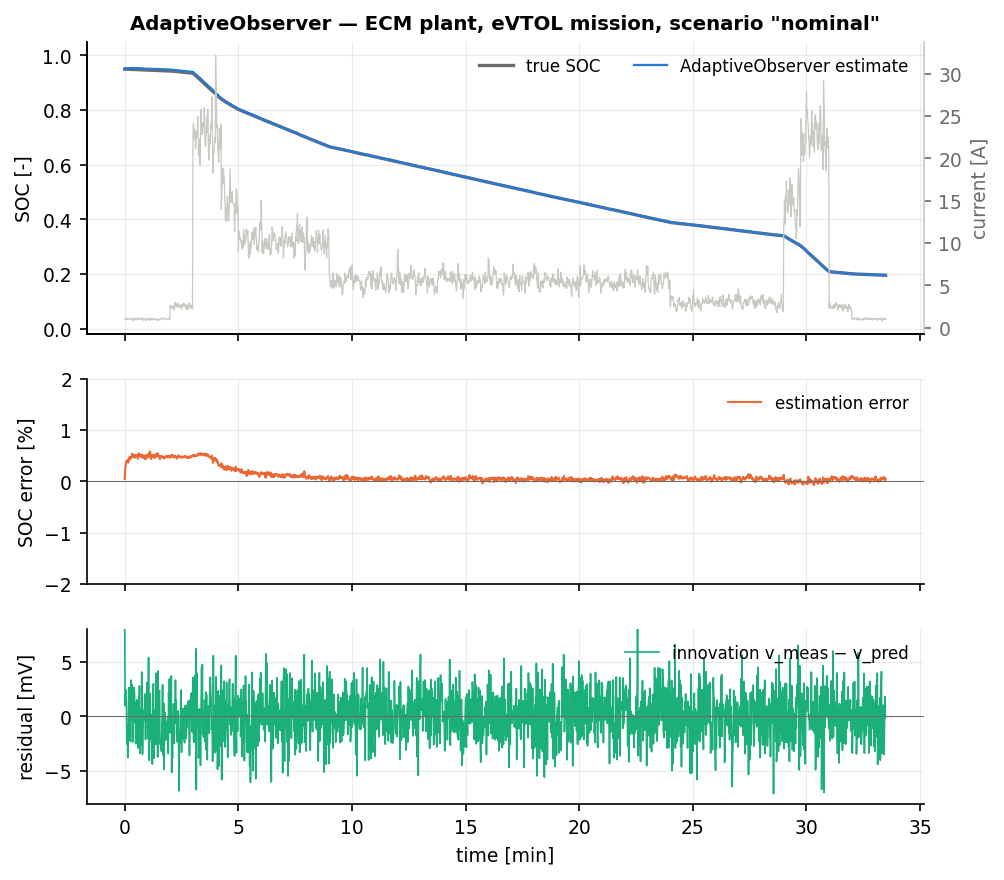
\includegraphics[width=\textwidth]{figures/cell_AdaptiveObserver_nominal.png}
\caption{AdaptiveObserver on the nominal eVTOL mission: true and estimated SOC (top), estimation error with the $\pm 2\sigma$ band when available (middle), voltage residual (bottom).}
\end{figure}
\begin{figure}[H]\centering
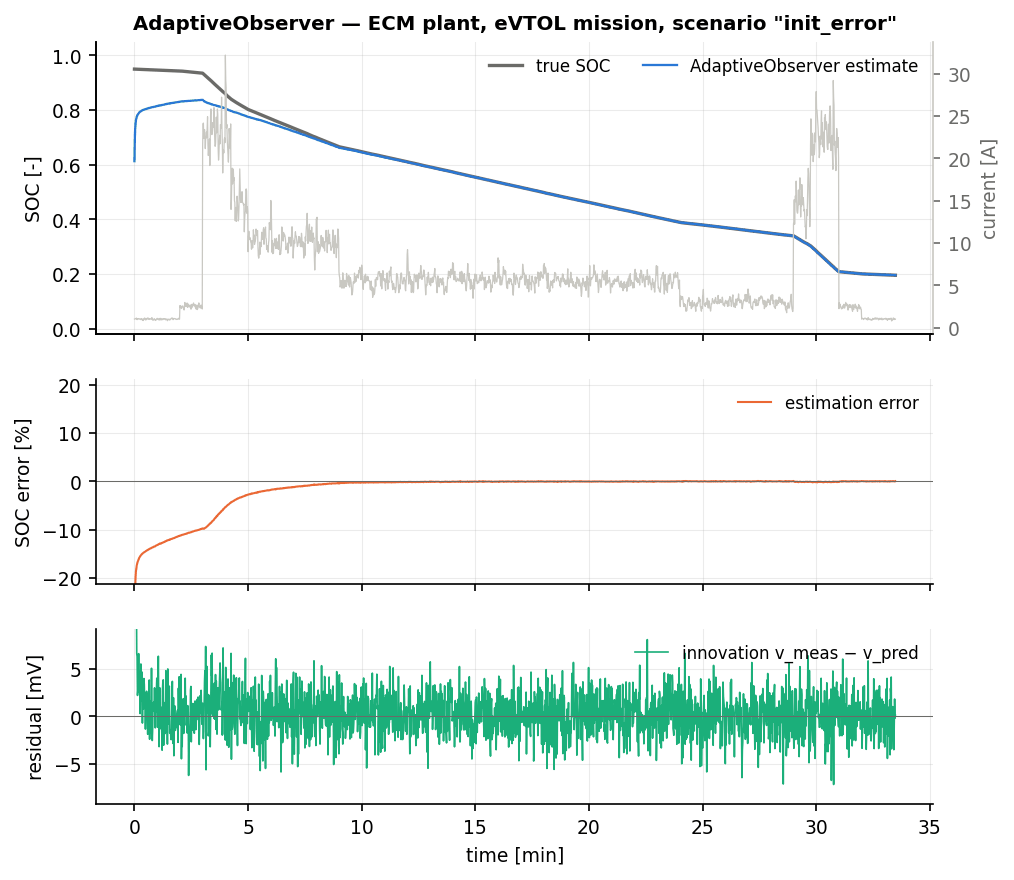
\includegraphics[width=\textwidth]{figures/cell_AdaptiveObserver_init_error.png}
\caption{AdaptiveObserver with a 35\,\% initial SOC error.}
\end{figure}

All numbers are over three seeds.  On the scenarios it is designed for, the adaptive observer is
the most accurate estimator in the study.  \texttt{aged\_cell} (true capacity $4.25$\,Ah,
estimator told $5.0$\,Ah) gives $\mathrm{rmse}_{ss} = 0.0113$, against the EKF's $0.0152$ and
every fixed-gain observer's $0.019$--$0.026$.  \texttt{param\_mismatch} ($R_0$ scaled by $0.7$)
gives $0.0083$ against the EKF's $0.0136$ --- a factor of $1.6$, and the best result on that
column of any method here.  \texttt{combined} gives $0.0080$ ($0.0078$--$0.0085$ across seeds)
against the EKF's $0.1244$ and the next-best observer's $0.0180$: with four simultaneous faults
the ability to move a parameter is worth more than any amount of gain design.  On the
single-particle plant it is the best observer in the family on \texttt{nominal} ($0.0045$) and
\texttt{cold} ($0.0179$), against the EKF's $0.0373$ and $0.0735$.

Steady-state accuracy on the well-posed scenarios is also strong: \texttt{nominal} $0.0005$
(equal to the EKF, and with $\hat{\bm{\phi}} = [-0.000,\,-0.004]$, i.e. the adaptation correctly
finds nothing to correct), \texttt{cold} $0.0025$, \texttt{outliers} $0.0017$,
\texttt{sensor\_dropout} $0.0007$.

\subsection*{What is identified, and what is not}
\label{sec:ad-ident}
The parameter estimates have to be reported carefully, because the honest result is more
interesting than the flattering one.  Measured at the end of the mission with the registered
gains:
\begin{center}
\begin{tabular}{@{}lccc@{}}
\toprule
scenario & $\hat{\bm{\phi}} = [\phi_Q,\ \phi_{R_0}]$ & $\hat{Q}_{Ah}$ (true) & $\hat{R}_0$ (true) \\
\midrule
\texttt{nominal}        & $[-0.000,\ -0.004]$ & $5.00$ ($4.98$) & $12.0$ ($12.0$)\,m$\Omega$ \\
\texttt{param\_mismatch} & $[-0.000,\ +0.137]$ & $5.00$ ($4.98$) & $\ \,9.6$ ($12.0$)\,m$\Omega$ \\
\texttt{aged\_cell}      & $[-0.000,\ +0.203]$ & $5.00$ ($4.23$) & $14.4$ ($12.0$)\,m$\Omega$ \\
\texttt{combined}       & $[-0.014,\ +0.211]$ & $4.93$ ($4.49$) & $14.5$ ($12.0$)\,m$\Omega$ \\
\bottomrule
\end{tabular}
\end{center}
Two things stand out.  On \texttt{param\_mismatch} the observer recovers about a third of the
$R_0$ error ($+13.7\,\%$ of the $+42.9\,\%$ it would need) --- real identification, and enough to
cut the SOC error by a factor of $1.6$, but not a calibration.  On \texttt{aged\_cell} the
capacity is \emph{not} identified at all; instead the observer explains the capacity loss as a
$+20\,\%$ increase in $R_0$, which is the wrong parameter but fits the voltage and halves the SOC
error.

This is a confound, and its cause is a direct consequence of the gain certification of
\Cref{sec:lue-schedule}.  A capacity error shows up as a slow drift of the SOC channel; the
sensitivity filter $\bm{\Upsilon}$ of \eqref{eq:ad-ups-pred} sees it only to the extent that the state
loop lets it accumulate, and its own recursion $\bm{\Upsilon}\leftarrow\bm{\Upsilon}-\mL\bm{\Omega}$
is driven by the same $\mL$.  A certified gain closes the SOC loop with a $30$\,s time constant,
so the drift is corrected long before the parameter can see it --- the state estimator hides the
very signal the parameter estimator needs.  An earlier version of this chapter reported
$\hat{Q}_{Ah}\to4.20$\,Ah against a true $4.25$, and that number was real, but it was obtained
with an \emph{uncertified} pole-placement gain whose SOC channel was effectively open
($L_{\soc}\approx10^{-4}$).  The same gain made the observer's sibling registrations diverge on two
seeds out of three on \texttt{combined}.  The capacity was identifiable because the state loop was
broken.

The trade was measured rather than assumed.  Sweeping the SOC process-noise allowance
$q_{\text{extra},\soc}$ downwards (which slows the certified LQE loop) does bring the capacity
back --- at $4\times10^{-5}$ and $\gamma_Q=2$, $\hat{Q}_{Ah}=4.86$\,Ah and \texttt{aged\_cell}
falls to $0.0024$ --- but it costs the \texttt{cold} scenario, whose worst seed goes from
$\mathrm{rmse}_{ss}=0.0025$ (max error $0.09$) to $0.0040$ with a $0.37$ transient, and at
$5\times10^{-5}$ with $\gamma_Q=2$ one seed reaches $0.162$ outright.  Raising $\gamma_Q$ at the
certified setting does not help: from $\gamma_Q=0.1$ to $100$, $\hat{Q}_{Ah}$ on
\texttt{aged\_cell} moves only from $5.00$ to $4.93$\,Ah, and $\gamma_Q=30$ already produces a
$0.38$ transient on \texttt{cold}.  The registered setting therefore keeps the certified loop and
accepts that the state-of-health output is not trustworthy on this mission.  This is the classical
dual-control tension --- a controller (or estimator) that regulates well stops exciting what it
would need in order to learn --- and it is worth stating that it survived every attempt to tune
around it.

The practical conclusion is that \texttt{capacity\_Ah()} from this observer should be read as a
diagnostic, not as a state-of-health measurement, unless the duty cycle contains a genuine
capacity-identifying excitation (a deep, slow discharge with rest periods) or the observer is run
with a deliberately detuned SOC channel during a dedicated characterisation.  The SOC estimate is
excellent either way; the parameter estimate is only as good as the excitation.

\section{Summary}
The adaptive observer is the only structure in this family that fixes the \emph{cause} of a
model-induced bias rather than compensating its effect, and on this benchmark it is three to six
accurate than every alternative on an aged cell, on a mis-identified $R_0$ and on the
four-fault \texttt{combined} scenario, where it beats the next-best observer by a factor of
$2.3$ and the EKF by a factor of $16$.  Adapt a dimensionless
relative deviation rather than the physical parameters, use per-parameter gains scaled inversely
to the excitation, normalise the gradient, project, and include Zhang's state/parameter coupling
term --- it is what makes the joint error dynamics triangular.  Gate the adaptation on the
residual magnitude if sensor faults are expected, and do not ask it to separate parameters that
the excitation does not separate: check the persistency of excitation of $\bm{\Omega}$ before
believing a state-of-health number.  Above all, be aware that the state loop and the parameter
loop compete for the same signal (\Cref{sec:ad-ident}): a well-certified observer corrects a slow
parameter-induced drift before the adaptation can see it, so a trustworthy capacity number needs
either an excitation the mission does not supply or a deliberately detuned state channel, and the
second of those buys the capacity back at the cost of robustness on cold cells.
